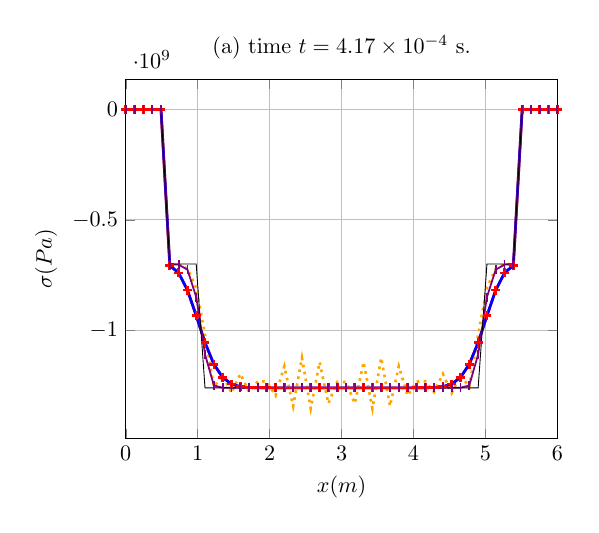
\begin{tikzpicture}[scale=0.8]
\begin{axis}[xlabel=$x (m)$,ylabel=$\sigma (Pa)$,ymajorgrids=true,xmajorgrids=true,legend pos=outer north east,title={(a) time $t = 4.17\times 10^{-4} $ s.},xmin=0.,xmax=6.]
\addplot[Red,very thick,mark=+,solid] coordinates {(0.0,-3.2561158711216654e-07) (0.12244897959183673,-6.54162606232603e-22) (0.24489795918367346,0.0) (0.36734693877551017,3.2561158711216643e-07) (0.4897959183673469,-4.884173806682499e-07) (0.6122448979591837,-706703995.0062007) (0.7346938775510203,-739923853.3127105) (0.8571428571428571,-818114621.3278772) (0.9795918367346939,-934350667.0858994) (1.1020408163265305,-1056745717.4113452) (1.2244897959183674,-1153785079.176232) (1.346938775510204,-1213891661.9862223) (1.4693877551020407,-1243675875.166416) (1.5918367346938775,-1255667377.4619899) (1.7142857142857142,-1259628756.7765899) (1.836734693877551,-1260708382.472525) (1.9591836734693877,-1260951555.06527) (2.0816326530612246,-1260996741.6987677) (2.204081632653061,-1261003631.246593) (2.326530612244898,-1261004484.7294881) (2.4489795918367347,-1261004569.3136225) (2.571428571428571,-1261004575.8625927) (2.693877551020408,-1261004576.2443771) (2.816326530612245,-1261004576.2601426) (2.9387755102040813,-1261004576.2605536) (3.061224489795918,-1261004576.2605536) (3.183673469387755,-1261004576.2601426) (3.306122448979592,-1261004576.2443776) (3.4285714285714284,-1261004575.862593) (3.5510204081632653,-1261004569.3136227) (3.673469387755102,-1261004484.7294881) (3.7959183673469385,-1261003631.2465928) (3.9183673469387754,-1260996741.6987677) (4.040816326530612,-1260951555.0652697) (4.163265306122449,-1260708382.4725246) (4.285714285714286,-1259628756.7765894) (4.408163265306122,-1255667377.4619899) (4.530612244897959,-1243675875.1664157) (4.653061224489796,-1213891661.9862223) (4.775510204081632,-1153785079.176232) (4.8979591836734695,-1056745717.4113454) (5.020408163265306,-934350667.0858992) (5.142857142857142,-818114621.327877) (5.26530612244898,-739923853.3127109) (5.387755102040816,-706703995.0062011) (5.5102040816326525,-4.884173806682498e-07) (5.63265306122449,0.0) (5.755102040816326,-4.884173806682498e-07) (5.877551020408163,0.0) (6.0,-4.884173806682498e-07) };
\addplot[Orange,very thick,mark=none,dotted] coordinates {(0.0011999999999999927,0.0) (0.12359999999999997,0.0) (0.24599999999999994,0.0) (0.36839999999999995,0.0) (0.4907999999999999,0.0) (0.6131999999999999,-700099961.461325) (0.7355999999999999,-702215400.6707044) (0.858,-720845446.6905135) (0.9803999999999998,-807249777.2239016) (1.1027999999999998,-1021817726.088786) (1.2251999999999996,-1257135415.8766613) (1.3475999999999997,-1201909815.2742617) (1.4699999999999998,-1284541316.0967622) (1.5923999999999996,-1197762497.5853782) (1.7147999999999997,-1280230396.1356874) (1.8371999999999995,-1230639248.475009) (1.9595999999999996,-1232614670.2907715) (2.0819999999999994,-1296340561.1434355) (2.2043999999999997,-1163180742.3691304) (2.3267999999999995,-1344085453.2920678) (2.4491999999999994,-1125286993.986051) (2.5715999999999997,-1354573027.5700727) (2.6939999999999995,-1144440690.6862848) (2.8163999999999993,-1331966839.3238678) (2.9387999999999996,-1234245710.8866477) (3.0611999999999995,-1234245710.8866642) (3.1835999999999993,-1331966839.3238637) (3.305999999999999,-1144440690.6862931) (3.4283999999999994,-1354573027.570076) (3.5507999999999993,-1125286993.9860492) (3.673199999999999,-1344085453.2920709) (3.7955999999999994,-1163180742.369132) (3.9179999999999993,-1296340561.143439) (4.040399999999999,-1232614670.2907667) (4.1628,-1230639248.4750104) (4.2852,-1280230396.1356888) (4.4076,-1197762497.5853772) (4.53,-1284541316.0967634) (4.6524,-1201909815.2742698) (4.7748,-1257135415.8766532) (4.8972,-1021817726.0887933) (5.0196,-807249777.2238963) (5.142,-720845446.6905184) (5.2644,-702215400.6706979) (5.3868,-700099961.4613259) (5.5092,0.0) (5.6316,0.0) (5.754,0.0) (5.8764,0.0) (5.9988,0.0) };
\addplot[Blue,very thick,mark=none,solid] coordinates {(0.0011999999999999927,0.0) (0.12359999999999997,0.0) (0.24599999999999994,0.0) (0.36839999999999995,0.0) (0.4907999999999999,0.0) (0.6131999999999999,-706703995.0062009) (0.7355999999999999,-739923853.3127103) (0.858,-818114621.3278768) (0.9803999999999998,-934350667.085899) (1.1027999999999998,-1056745717.4113449) (1.2251999999999996,-1153785079.176232) (1.3475999999999997,-1213891661.9862218) (1.4699999999999998,-1243675875.1664155) (1.5923999999999996,-1255667377.4619896) (1.7147999999999997,-1259628756.7765894) (1.8371999999999995,-1260708382.4725244) (1.9595999999999996,-1260951555.06527) (2.0819999999999994,-1260996741.6987672) (2.2043999999999997,-1261003631.246593) (2.3267999999999995,-1261004484.7294877) (2.4491999999999994,-1261004569.3136225) (2.5715999999999997,-1261004575.862593) (2.6939999999999995,-1261004576.2443774) (2.8163999999999993,-1261004576.2601426) (2.9387999999999996,-1261004576.2605534) (3.0611999999999995,-1261004576.2605536) (3.1835999999999993,-1261004576.2601426) (3.305999999999999,-1261004576.2443774) (3.4283999999999994,-1261004575.862593) (3.5507999999999993,-1261004569.3136225) (3.673199999999999,-1261004484.729488) (3.7955999999999994,-1261003631.246593) (3.9179999999999993,-1260996741.6987672) (4.040399999999999,-1260951555.06527) (4.1628,-1260708382.4725244) (4.2852,-1259628756.7765892) (4.4076,-1255667377.4619894) (4.53,-1243675875.1664155) (4.6524,-1213891661.9862218) (4.7748,-1153785079.1762319) (4.8972,-1056745717.4113448) (5.0196,-934350667.0858989) (5.142,-818114621.3278767) (5.2644,-739923853.3127103) (5.3868,-706703995.0062009) (5.5092,0.0) (5.6316,0.0) (5.754,0.0) (5.8764,0.0) (5.9988,0.0) };
\addplot[Purple,thick,mark=|,solid] coordinates {(0.0011999999999999927,0.0) (0.12359999999999997,0.0) (0.24599999999999994,0.0) (0.36839999999999995,0.0) (0.4907999999999999,0.0) (0.6131999999999999,-700149009.8511133) (0.7355999999999999,-702792255.866507) (0.858,-725326867.326901) (0.9803999999999998,-850156660.8530495) (1.1027999999999998,-1109984935.9712873) (1.2251999999999996,-1250258832.4370122) (1.3475999999999997,-1260471082.9558206) (1.4699999999999998,-1260981625.9873586) (1.5923999999999996,-1261003693.8957453) (1.7147999999999997,-1261004546.9659622) (1.8371999999999995,-1261004575.4299965) (1.9595999999999996,-1261004576.2405941) (2.0819999999999994,-1261004576.260158) (2.2043999999999997,-1261004576.2605524) (2.3267999999999995,-1261004576.260559) (2.4491999999999994,-1261004576.260559) (2.5715999999999997,-1261004576.260559) (2.6939999999999995,-1261004576.260559) (2.8163999999999993,-1261004576.2605588) (2.9387999999999996,-1261004576.2605588) (3.0611999999999995,-1261004576.260559) (3.1835999999999993,-1261004576.2605588) (3.305999999999999,-1261004576.2605588) (3.4283999999999994,-1261004576.2605588) (3.5507999999999993,-1261004576.2605588) (3.673199999999999,-1261004576.2605588) (3.7955999999999994,-1261004576.260553) (3.9179999999999993,-1261004576.2601585) (4.040399999999999,-1261004576.2405944) (4.1628,-1261004575.4299967) (4.2852,-1261004546.9659626) (4.4076,-1261003693.895745) (4.53,-1260981625.987358) (4.6524,-1260471082.955823) (4.7748,-1250258832.4370096) (4.8972,-1109984935.971287) (5.0196,-850156660.8530501) (5.142,-725326867.326901) (5.2644,-702792255.866507) (5.3868,-700149009.8511133) (5.5092,0.0) (5.6316,0.0) (5.754,0.0) (5.8764,0.0) (5.9988,0.0) };
\addplot[black,thin,mark=none,solid] coordinates {(0.0,-0.0) (0.12244897959183673,-0.0) (0.24489795918367346,-0.0) (0.36734693877551017,-0.0) (0.4897959183673469,-0.0) (0.6122448979591837,-700000000.0) (0.7346938775510203,-700000000.0) (0.8571428571428571,-700000000.0) (0.9795918367346939,-700000000.0) (1.1020408163265305,-1261004576.260559) (1.2244897959183674,-1261004576.260559) (1.346938775510204,-1261004576.260559) (1.4693877551020407,-1261004576.260559) (1.5918367346938775,-1261004576.260559) (1.7142857142857142,-1261004576.260559) (1.836734693877551,-1261004576.260559) (1.9591836734693877,-1261004576.260559) (2.0816326530612246,-1261004576.260559) (2.204081632653061,-1261004576.260559) (2.326530612244898,-1261004576.260559) (2.4489795918367347,-1261004576.260559) (2.571428571428571,-1261004576.260559) (2.693877551020408,-1261004576.260559) (2.816326530612245,-1261004576.260559) (2.9387755102040813,-1261004576.260559) (3.061224489795918,-1261004576.260559) (3.183673469387755,-1261004576.260559) (3.306122448979592,-1261004576.260559) (3.4285714285714284,-1261004576.260559) (3.5510204081632653,-1261004576.260559) (3.673469387755102,-1261004576.260559) (3.7959183673469385,-1261004576.260559) (3.9183673469387754,-1261004576.260559) (4.040816326530612,-1261004576.260559) (4.163265306122449,-1261004576.260559) (4.285714285714286,-1261004576.260559) (4.408163265306122,-1261004576.260559) (4.530612244897959,-1261004576.260559) (4.653061224489796,-1261004576.260559) (4.775510204081632,-1261004576.260559) (4.8979591836734695,-1261004576.260559) (5.020408163265306,-700000000.0) (5.142857142857142,-700000000.0) (5.26530612244898,-700000000.0) (5.387755102040816,-700000000.0) (5.5102040816326525,-0.0) (5.63265306122449,-0.0) (5.755102040816326,-0.0) (5.877551020408163,-0.0) (6.0,-0.0) };
%\legend{dgmpm,fem,fvm,fvm (SB),exact}
\end{axis}
\end{tikzpicture}
%%% Local Variables:
%%% mode: latex
%%% TeX-master: "../../mainManuscript"
%%% End:
